% Compile: xelatex proposal.tex && xelatex proposal.tex  (twice!)
\documentclass[12pt,a4paper]{article}
\usepackage[margin=1in]{geometry}
\usepackage{fontspec}
\setmainfont{Times New Roman}
\usepackage{amsmath,amssymb}
\usepackage{setspace,enumitem,titlesec}
\usepackage{tikz}
\usepackage[hidelinks]{hyperref}
\hypersetup{pdftitle={Verified Lie Reduction and Error Bounds for a Cubic Saint--Venant--Exner System}}
\doublespacing
\titleformat{\section}{\normalfont\normalsize\bfseries}{\thesection.}{0.5em}{}
\titlespacing*{\section}{0pt}{6pt}{0pt}
\titleformat{\subsection}{\normalfont\normalsize\bfseries}{}{0pt}{}
\titlespacing*{\subsection}{0pt}{6pt}{0pt}
\setlist[enumerate]{leftmargin=1.7em,itemsep=0pt,parsep=0pt,topsep=0pt}
\setlength{\parindent}{0pt}
\setlength{\parskip}{3pt}
\setlength{\emergencystretch}{2em}
\pagestyle{plain}
\newcommand{\R}{\mathbb{R}}
\newcommand{\pr}{\operatorname{pr}}
\begin{document}

\begin{center}
\textbf{Verified Lie Reduction and Error Bounds for a Cubic Saint--Venant--Exner System}

Research proposal\\
Carl \quad WKU MATH 4890\\
Proposed supervisor: Dr. Puneet Rana
\end{center}

\section{Research problem and rationale}
Nonlinear fluid equations often resist explicit solution, while numerical approximations can obscure the analytical structure of selected solution families. Lie symmetry offers a systematic route from a PDE to an invariant ansatz and a reduced equation. This project asks whether the reduction of a coupled shallow-water and sediment-transport system can be made coordinate-consistent, and whether the resulting profile can be approximated with a computable error bound.

The model is a one-dimensional Saint--Venant--Exner (SVE) system coupling shallow-water flow to bed evolution, with sediment flux $Q=A_g u^3$. Paliathanasis, Leon and Leach \cite{sve} analysed a related scalar equation in Lagrange variables and reported a five-dimensional symmetry algebra at the exceptional exponent $m=3$. This proposal does not repeat that classification. It audits the coordinate transformation, adopts one convention explicitly, and verifies each reported generator on the coordinate-consistent equation.

\textbf{Thesis.} For the cubic SVE on a bounded spatio-temporal domain, we construct a coordinate-consistent travelling-wave reduction, compute the approximate symmetry algebra at $m=3+\delta$, and bound the error of a semi-analytical approximation to the reduced profile. A neural remainder is tested as a hypothesis; a negative result is an acceptable outcome.

The key innovation is the combination of two ideas. First, we treat $m$ as a perturbed quantity $m=3+\delta$, so that the exceptional symmetry $X_5$ becomes an \emph{approximate} symmetry in the sense of Baikov--Gazizov--Ibragimov \cite{bgi}. Second, we transfer the Gronwall-type error estimate from the reduced ODE to the reconstructed fields $(h,u,B)$, providing a certificate that is computable from the profile alone. Neither idea is new in isolation; the contribution is their verified combination on this model.

\section{Model, scope, and objectives}
For smooth fields $(h,u,B)$ on $(t,x)\in(0,T)\times(0,L)$,
\begin{equation}
\begin{aligned}
h_t+(hu)_x&=0,\\
u_t+uu_x+g(h_x+B_x)&=0,\\
B_t+\xi\,A_g\,(u^3)_x&=0,
\end{aligned}
\label{eq:sve}
\end{equation}
where $h>0$ is depth, $u$ velocity, $B$ bed elevation, $g>0$ gravity, $A_g>0$ a transport coefficient, and $\xi=(1-p)^{-1}$ accounts for bed porosity $p\in[0,1)$. We restrict to $u>0$. No drag term is introduced: weak linear drag breaks the scaling symmetry on which the Lagrange reduction rests. Periodic boundary conditions are used, with data given by the trace of a similarity solution.

The objectives are:
\begin{enumerate}
\item Audit the Eulerian-to-Lagrangian transformation of \eqref{eq:sve}, including the transport term that arises when bed elevation is evaluated along water-particle paths.
\item Adopt one coordinate convention explicitly, derive the resulting master equation, and verify the generators reported in \cite{sve} on it.
\item Compute the approximate symmetry algebra at $m=3+\delta$ using the Baikov--Gazizov--Ibragimov framework \cite{bgi} and the consistent approach of Di Salvo, Gorgone and Oliveri \cite{disalvo}.
\item Construct a travelling-wave reduction $\sigma=x-ct$ and reduce \eqref{eq:sve} to a regular ODE system.
\item Derive a computable error envelope for the reconstructed fields $h,u,B$ on a specified regular interval.
\item Test whether a neural series remainder improves the truncated-series approximation at matched cost.
\end{enumerate}
Global shocks, dry beds, drag, and two-dimensional extensions lie outside the scope.

\section{Methodology I: coordinate audit and Lie reduction}

\subsection*{Coordinate transformation and master equation}
Let $x=\phi(t,s)$ give the position at time $t$ of the water element labelled by mass coordinate $s$, so that $\phi_t=u(t,\phi)$ and $\phi_s=1/h(t,\phi)>0$. For any Eulerian field $f$, define the pullback $\tilde f(t,s)=f(t,\phi(t,s))$. The chain rule gives
\begin{equation}
\partial_x=\phi_s^{-1}\partial_s,\qquad
(\partial_t)_x=(\partial_t)_s-\frac{\phi_t}{\phi_s}\partial_s.
\label{eq:chain}
\end{equation}
Applying \eqref{eq:chain} to the Exner equation in \eqref{eq:sve} gives
\begin{equation}
\tilde B_t-\frac{\phi_t}{\phi_s}\tilde B_s+\beta\,(\phi_t)^{2}\frac{\phi_{ts}}{\phi_s}=0,
\qquad \beta=3\xi A_g,
\label{eq:bed}
\end{equation}
while the momentum balance becomes
\begin{equation}
\phi_{tt}-g\frac{\phi_{ss}}{\phi_s^{3}}+\frac{g}{\phi_s}\tilde B_s=0.
\label{eq:mom}
\end{equation}
The transport term $-(\phi_t/\phi_s)\tilde B_s$ in \eqref{eq:bed} is absent from the printed equation of \cite{sve}. We resolve this by direct derivation from \eqref{eq:sve} and record the resolution explicitly.

We adopt the \emph{physical pullback} convention, in which $\tilde B$ is the bed elevation evaluated along the water-parcel path. Under this convention, \eqref{eq:bed} and \eqref{eq:mom} specify the two derivatives of $\tilde B$. Mixed-derivative compatibility $\tilde B_{st}=\tilde B_{ts}$ yields the scalar master equation
\begin{equation}
\mathcal F[\phi]=\partial_t\!\left(\frac{\phi_s}{g}A\right)
-\partial_s\!\left(\frac{\phi_t}{g}A\right)+\beta\,\partial_s S=0,
\label{eq:master}
\end{equation}
where
\begin{equation}
A=\phi_{tt}-g\frac{\phi_{ss}}{\phi_s^{3}},\qquad
S=(\phi_t)^{2}\frac{\phi_{ts}}{\phi_s}.
\end{equation}
Equation \eqref{eq:master} differs from the printed master equation of \cite{sve} precisely by the transport terms inherited from \eqref{eq:bed}.

\begin{center}
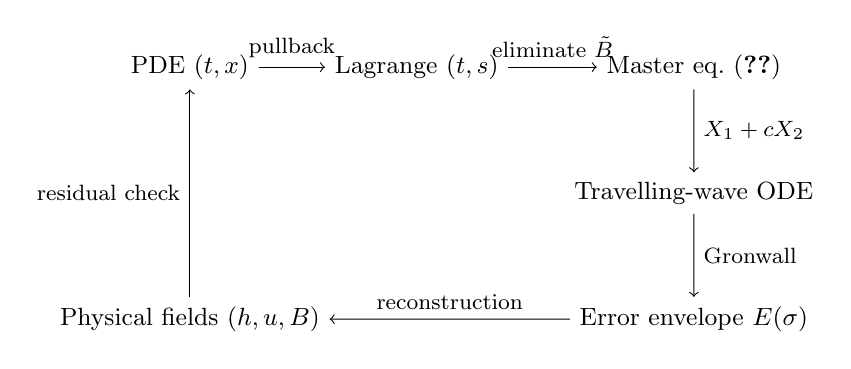
\begin{tikzpicture}[scale=0.8, every node/.style={font=\small}]
  \node (pde) at (0,0) {PDE $(t,x)$};
  \node (lag) at (3.6,0) {Lagrange $(t,s)$};
  \node (master) at (8,0) {Master eq.\ \eqref{eq:master}};
  \node (ode) at (8,-2) {Travelling-wave ODE};
  \node (bound) at (8,-4) {Error envelope $E(\sigma)$};
  \node (phys) at (0,-4) {Physical fields $(h,u,B)$};
  \draw[->] (pde) -- node[above]{\footnotesize pullback} (lag);
  \draw[->] (lag) -- node[above]{\footnotesize eliminate $\tilde B$} (master);
  \draw[->] (master) -- node[right]{\footnotesize $X_1+cX_2$} (ode);
  \draw[->] (ode) -- node[right]{\footnotesize Gronwall} (bound);
  \draw[->] (bound) -- node[above]{\footnotesize reconstruction} (phys);
  \draw[->] (phys) -- node[left]{\footnotesize residual check} (pde);
\end{tikzpicture}
\end{center}

\subsection*{Symmetry verification and approximate symmetry at $m=3+\delta$}
We do not redo the group classification. At $\delta=0$, we verify the five generators reported in \cite{sve} on \eqref{eq:master}: the three translations/scalings
\[
X_1=\partial_t,\quad X_2=\partial_s,\quad X_3=t\partial_t+s\partial_s,
\]
the bed translation $X_4=\partial_{\tilde B}$ (realised indirectly through \eqref{eq:bed}--\eqref{eq:mom}), and the exceptional generator
\[
X_5=t\partial_t-2\phi_t\partial_{\phi_t}-2\tilde B\partial_{\tilde B}
\]
at $m=3$. For each candidate $X_i$, we compute $\pr^{(3)}X_i(\mathcal F)|_{\mathcal F=0}$ by exact rational arithmetic using SymPy's prolongation formula.

At $m=3+\delta$, $X_5$ is no longer exact. Following \cite{bgi}, we seek an approximate symmetry
\[
X_5^\delta=X_5+\delta\,X_5^{(1)}+O(\delta^2)
\]
satisfying $\pr^{(3)}X_5^\delta(\mathcal F_\delta)|_{\mathcal F_\delta=0}=O(\delta^2)$, where $\mathcal F_\delta$ is \eqref{eq:master} with $m=3+\delta$. The commutator closure becomes
\[
[X_5^\delta,X_i]=\sum_j c_{5i}^j X_j+\delta\sum_j c_{5i}^{(1)j}X_j+O(\delta^2).
\]
The corrected structure constants $c_{5i}^{(1)j}$ measure how the exceptional symmetry deforms. We report $\dim\mathfrak g_\delta$ as a function of $\delta$, producing a discrete bifurcation at $\delta=0$.

\begin{center}
\begin{tikzpicture}[scale=0.85]
  \draw[->] (0,0) -- (5.2,0) node[right]{$m$};
  \draw[->] (0,0) -- (0,3) node[above]{$\dim\mathfrak g(m)$};
  \draw[thick] (0,1.1) -- (3,1.1);
  \draw[thick] (3,1.1) -- (3,2.2);
  \draw[thick] (3,2.2) -- (4.9,2.2);
  \node at (1.5,0.65) {\footnotesize 4};
  \node at (4.0,2.55) {\footnotesize 5};
  \draw[dashed] (3,0) -- (3,2.2);
  \node at (3,-0.35) {\footnotesize $m=3$};
\end{tikzpicture}
\end{center}

\subsection*{Travelling-wave reduction and dynamical systems}
We select $X_1+cX_2$ with invariant variable $\sigma=s-ct$. Its action on the independent variables has rank one, and the invariant-surface condition
\[
\eta-\tau\phi_t-\xi\phi_s=0
\]
admits a nonconstant graph. Substitution into \eqref{eq:master} collapses the two independent variables to one. Unlike the scaling ansatz $\phi=t\Phi(s/t)$, this reduction does not depend on transport-term cancellation; it is therefore compatible with the physical pullback convention. The reduced problem is a third-order ODE in $\sigma$, which we integrate once to obtain a second-order system with a conserved constant $C$.

Setting $y=(\phi,\phi_\sigma,\phi_{\sigma\sigma})$, the reduced equation defines a three-dimensional continuous dynamical system $y'=f(y;C)$. We analyse fixed points (uniform-flow states), their Jacobians, and the Lipschitz constant $L=\sup\|Df\|_\infty$ on a tube around a reference orbit. This constant feeds directly into \S4.

\section{Methodology II: series construction and error certificate}

\subsection*{Local series and reconstruction}
Let $y(\sigma)=\sum_{k\ge 0}a_k(\sigma-\sigma_0)^k$ solve the reduced ODE near a regular point $\sigma_0$. Coefficients satisfy a recurrence from formal division, analytic where the denominator is bounded away from zero. We compute coefficients up to order $N$ symbolically. For $h=1/\phi_s$ and $u=\phi_t$, the error envelopes transfer as
\[
|\hat h-h|\le E/\delta^2,\qquad
|\hat u-u|\le(1+|\sigma|)E,\qquad
|\hat B-B|\le E,
\]
where $\delta>0$ bounds $\phi_s$ from below on the interval.

\subsection*{A posteriori error envelope}
Let $\hat y$ be a differentiable approximation and $r(\sigma)=\hat y'(\sigma)-f(\sigma,\hat y(\sigma))$ its residual.

\textbf{Proposition.} Fix $I=[\sigma_0,\sigma_0+\ell]$ and a tube of radius $R$ around $\hat y$. Suppose (i) $f$ is $L$-Lipschitz on the tube; (ii) $\|r\|_{L^\infty(I)}\le\epsilon$; (iii) $\|\hat y(\sigma_0)-y(\sigma_0)\|_\infty\le\epsilon_0$. Then
\[
\|\hat y(\sigma)-y(\sigma)\|_\infty\le E(\sigma-\sigma_0)
:=\Big(\epsilon_0+\frac{\epsilon}{L}\Big)e^{L(\sigma-\sigma_0)}-\frac{\epsilon}{L},
\]
provided $E(\sigma-\sigma_0)<R$ on $I$. We compute $L$ from \S3.3 and $\epsilon$ from interval arithmetic or a polynomial remainder bound. Floating-point samples alone do not establish a supremum bound; the tube condition is checked explicitly.

\subsection*{Optional neural remainder}
After the analytical certificate is in place, we test the trial function
\[
\hat y_\theta(\sigma)=P_N(\sigma)+(\sigma-\sigma_0)^{N+1}\mathcal N_\theta(\sigma)
\]
with a small feedforward network $\mathcal N_\theta$. Training minimises the coefficient residual, not the full squared residual, so a small $\epsilon$ cannot mask an inaccurate correction. We report whether the neural remainder reduces the $L^2$ error at matched cost; a negative result is informative.

\section{Evaluation, expected outcomes, and work plan}
Compare four methods on the same branch: truncated series; adaptive classical ODE solver; neural ODE without series structure; hybrid series-plus-neural. Report:
\begin{itemize}
\item relative $L^2$ and maximum errors in reduced and reconstructed fields;
\item residuals of the reconstructed original balances \eqref{eq:sve};
\item admissibility violations ($h\le 0$, singular denominators);
\item training time, inference time, and query cost.
\end{itemize}
Reference accuracy is checked by tolerance refinement. Networks use matched budgets, multiple seeds, and evaluation points distinct from training points.

\textbf{Expected outcomes.} A coordinate audit with a stated convention; verified generators on the corrected master equation; an approximate-symmetry computation at $m=3+\delta$ with a bifurcation diagram; a travelling-wave reduction with a regular branch; a computable error envelope; and a fair comparison identifying when the neural remainder helps or fails.

\textbf{Twelve-week plan.} Weeks 1--2: coordinate audit and verification of \eqref{eq:master}. Weeks 3--4: verification of the five generators and approximate-symmetry computation. Weeks 5--6: travelling-wave reduction and dynamical-systems analysis. Weeks 7--8: series construction and certificate. Weeks 9--10: neural remainder experiments. Weeks 11--12: evaluation and writing.

\subsection*{Risks and mitigations}
\begin{enumerate}
\item \textbf{Coordinate convention disagreement.} Resolve by direct derivation from \eqref{eq:sve} and record both conventions; report the difference without claiming an error.
\item \textbf{Approximate symmetry computation too heavy.} Limit to polynomial coefficients of degree $\le D$; report the stabilization degree; if the algebra does not close to first order in $\delta$, report the obstruction.
\item \textbf{Gronwall bound vacuous.} Compute $L,\epsilon$ on short subintervals; if the bound exceeds $R$, report the failure and shrink the interval.
\item \textbf{Neural remainder fails to improve.} Report the negative result with matched budgets and multiple seeds; it does not invalidate the certificate.
\end{enumerate}

\begin{thebibliography}{9}
\raggedright
\setlength{\itemsep}{3pt}
\setlength{\parskip}{0pt}
\bibitem{sve}
A. Paliathanasis, G. Leon, and P. G. L. Leach.
``Lie Symmetries and Similarity Solutions for a Shallow-Water Model with Bed Elevation in Lagrange Variables.''
\emph{Mathematics}, 14(3), 433, 2026.
\href{https://doi.org/10.3390/math14030433}{doi:10.3390/math14030433}.

\bibitem{sve2022}
A. Paliathanasis.
``Lie Symmetry Analysis of the One-Dimensional Saint-Venant--Exner Model.''
\emph{Symmetry}, 14(8), 1679, 2022.
\href{https://doi.org/10.3390/sym14081679}{doi:10.3390/sym14081679}.

\bibitem{bgi}
V. A. Baikov, R. K. Gazizov, and N. Kh. Ibragimov.
``Approximate symmetries.''
\emph{Mathematics of the USSR-Sbornik}, 64(2), 427--441, 1989.
\href{https://doi.org/10.1070/SM1989v064n02ABEH003318}{doi:10.1070/SM1989v064n02ABEH003318}.

\bibitem{disalvo}
R. Di Salvo, M. Gorgone, and F. Oliveri.
``A consistent approach to approximate Lie symmetries of differential equations.''
\emph{Nonlinear Dynamics}, 91(1), 371--386, 2018.
\href{https://arxiv.org/abs/2108.02169}{arXiv:2108.02169}.

\bibitem{patera}
J. Patera and P. Winternitz.
``Subalgebras of real three- and four-dimensional Lie algebras.''
\emph{Journal of Mathematical Physics}, 18(7), 1449--1455, 1977.

\bibitem{olver}
P. J. Olver. \emph{Applications of Lie Groups to Differential Equations}.
Second edition, Springer, 1993.

\bibitem{lagaris}
I. E. Lagaris, A. Likas, and D. I. Fotiadis.
``Artificial Neural Networks for Solving Ordinary and Partial Differential Equations.''
\emph{IEEE Transactions on Neural Networks}, 9(5), 987--1000, 1998.

\bibitem{pinn}
S. Cuomo et al.
``Scientific Machine Learning Through Physics--Informed Neural Networks: Where we are and What's Next.''
\emph{Journal of Scientific Computing}, 92, 88, 2022.

\bibitem{hillebrecht}
B. Hillebrecht and B. Unger.
``Certified machine learning: A posteriori error estimation for physics-informed neural networks.''
\emph{IJCNN}, 2022.
\href{https://doi.org/10.1109/IJCNN55064.2022.9892569}{doi:10.1109/IJCNN55064.2022.9892569}.
\end{thebibliography}
\end{document}